
It has been shown that the number of charged particles with transverse
momentum (\pT ) above 500\,MeV, \ntrk, associated with a jet can be used
to select samples which have an increased fraction of jets produced by
quarks (or gluons). Samples with enhanced fractions of quark or gluon
initiated jets can be created by using a selection based on the \ntrk\
as shown in Fig.~\ref{fig:jet_pt_quark_gluon}.
Ref.~\cite{ATL-PHYS-PUB-2017-009} also shows that the \Pythia8
generator~\cite{pythia8} using the A14 tune~\cite{A14tune} is in a good
agreement with the distribution of \ntrk\ found in data.


\begin{figure}[htb]
 \centering
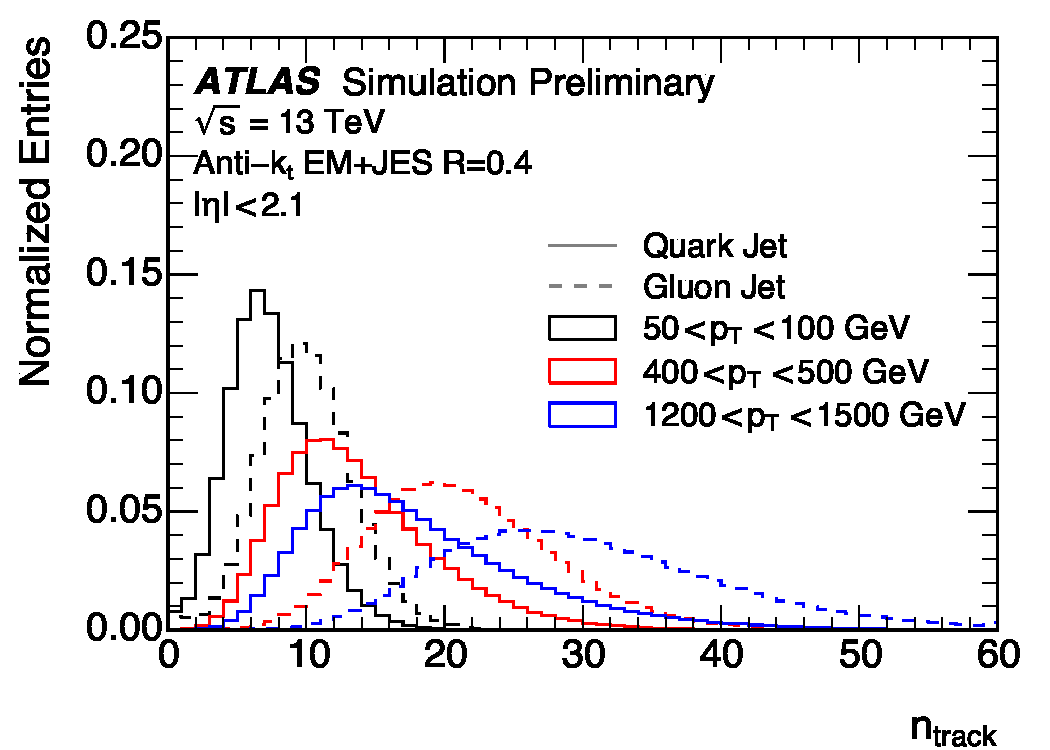
\includegraphics[width=0.75\textwidth]{figures/tagging/fig_01_ATL-PHYS-PUB-2017-009.pdf}
\caption{Distribution of the jet reconstructed track multiplicity (\ntrk ) in
 different pT ranges with the \Pythia~8 generator~\cite{pythia8} using
 the A14 tune~\cite{A14tune}, the NNPDF2.3 PDF
 set~\cite{Carrazza:2013axa}, and processes with a full simulation of the
 ATLAS detector. Jets must be fully within the tracking acceptance
 ($|\eta|<2.1$) and tracks are required to have $\pT > 500$\,MeV and pass
  quality criteria described in Ref.~\cite{ATL-PHYS-PUB-2017-009}. Figure
 from Ref.~\cite{ATL-PHYS-PUB-2017-009}. \label{fig:jet_pt_quark_gluon}}
\end{figure}

In Ref.~\cite{ATL-PHYS-PUB-2017-009}  the selection criteria for  an
enriched quark-initiated jet sample was chosen so that each \pT\ bin had
60\% quark-initiated purity. Applying this criteria to the high mass
dijet sample would lead to discontinuities in the mass spectrum that
would present difficulties to a resonance search. 

Using a selection criteria that is a linear function of the \( \ln \pT \) 
results in a smooth mass distribution and can be chosen to produce a uniform 
selection efficiency.  A jet is classed as being quark-initiated if \ntrk is less than
the threshold \nq and a gluon-initiated if \ntrk is greater than the threshold \ngluon  
\begin{align}
\ntrk & \le \nq \; \mbox{quark-initiated sample} \label{eq:QGselect} \\
\ntrk	  & \ge \ngluon \; \mbox{gluon-initiated sample} \nonumber
\end{align}
where   
\begin{equation}
n_{\mathrm{q(g)}} = {m \ln(\pT) + c}  \label{eq:nqg2}
\end{equation}
where $m$ and $c$ are constants chosen to provide suitable subsamples.

The constants $m$ and $c$ are found by finding the value of \ntrk\ 
that corresponds to a given efficiency for truth quark and gluon jets in 
\pT\ bins and fitting the results. The jet \pT\ bin edges are chosen to be 
400, 500, 650, 800, 1000, 1200, 1500, 2000, 3000, 6000\,\GeV. An example of the \ntrk cumulative 
distribution for truth quark and gluon jets satisfying $800 < \pT < 1000\,\GeV$ is shown in
Fig.~\ref{fig:ntrk_cumulative}.


\begin{figure}[htb]
 \centering
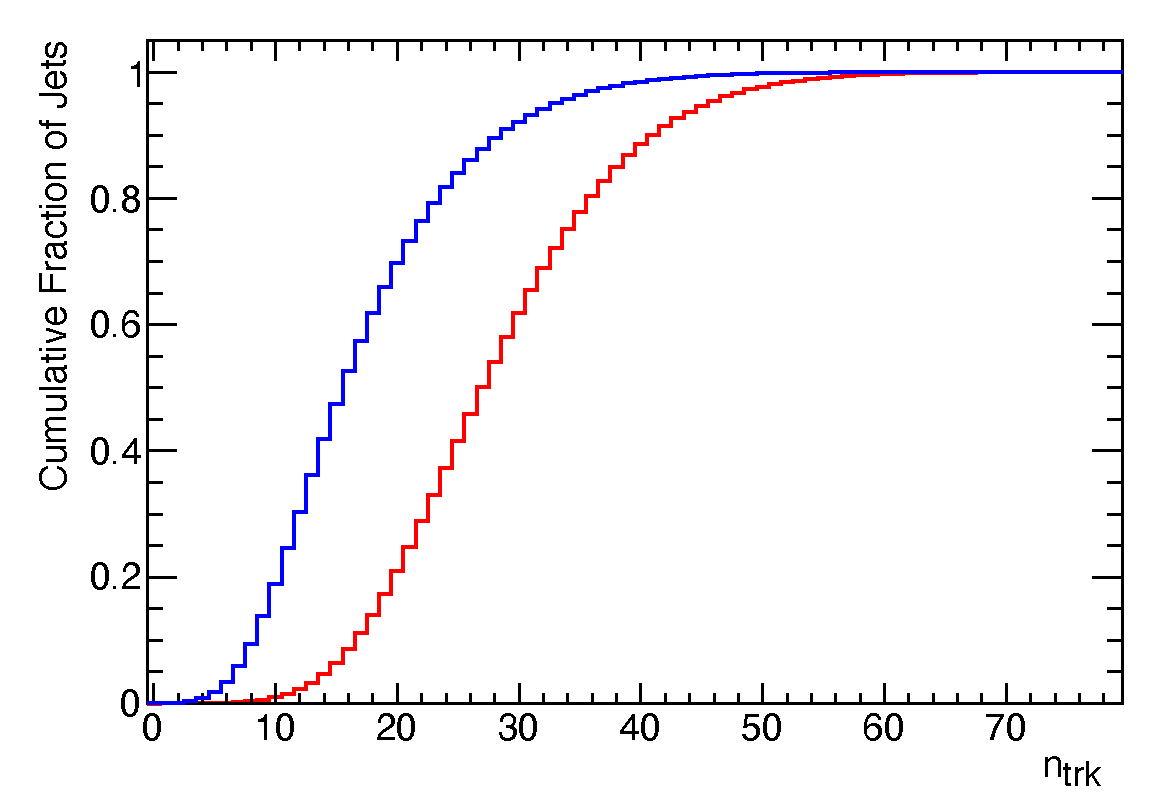
\includegraphics[width=0.75\textwidth]{figures/tagging/Cumulative_ntrk_distribution_4_800_1000GeV.pdf}
\caption{The cumulative distribution of \ntrk\ for truth quark (blue) and gluon (red) initiated jets 
satisfying $800 < \pT < 1000\,\GeV$.  \label{fig:ntrk_cumulative}}
\end{figure}


The constants for Eq.~\ref{eq:nqg2} are found for quark and gluon selection efficiencies from 
65\% to 95\% in 5\% steps. The plot of the value of \ntrk\ that satisfies the selection efficiencies 
of 70 and 80\% are shown in Fig.~\ref{fig:qg_selection_curves} along with the best fit using Eq.~\ref{eq:nqg2}.
The values of the constants for both quark and gluon selections are summarised in 
Tables~\ref{table:truthQuarkSelectionEfficiencies} and \ref{table:truthGluonSelectionEfficiencies}.

\begin{figure}[htb]
 \centering
  \subfigure[] {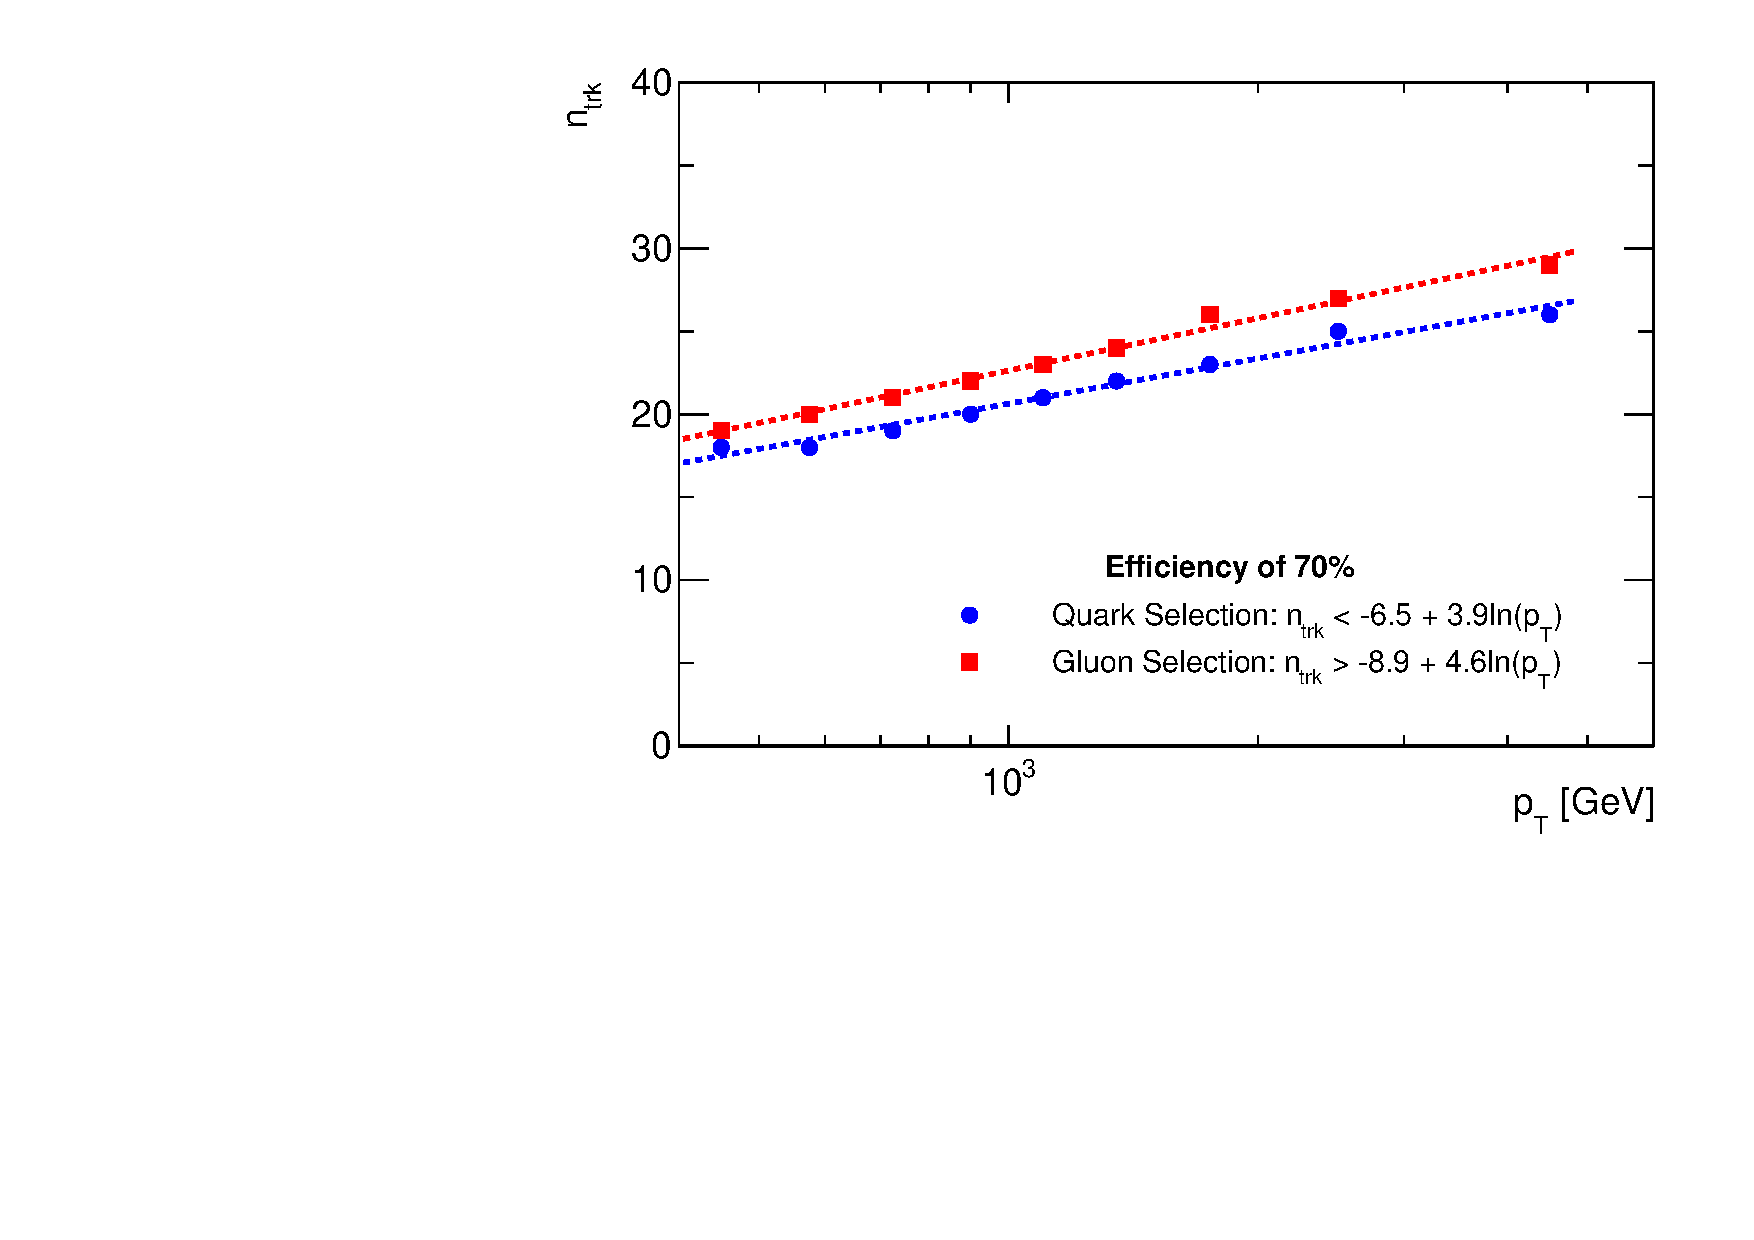
\includegraphics[width=0.495\textwidth]{figures/tagging/quark_selection_6}}
  \subfigure[] {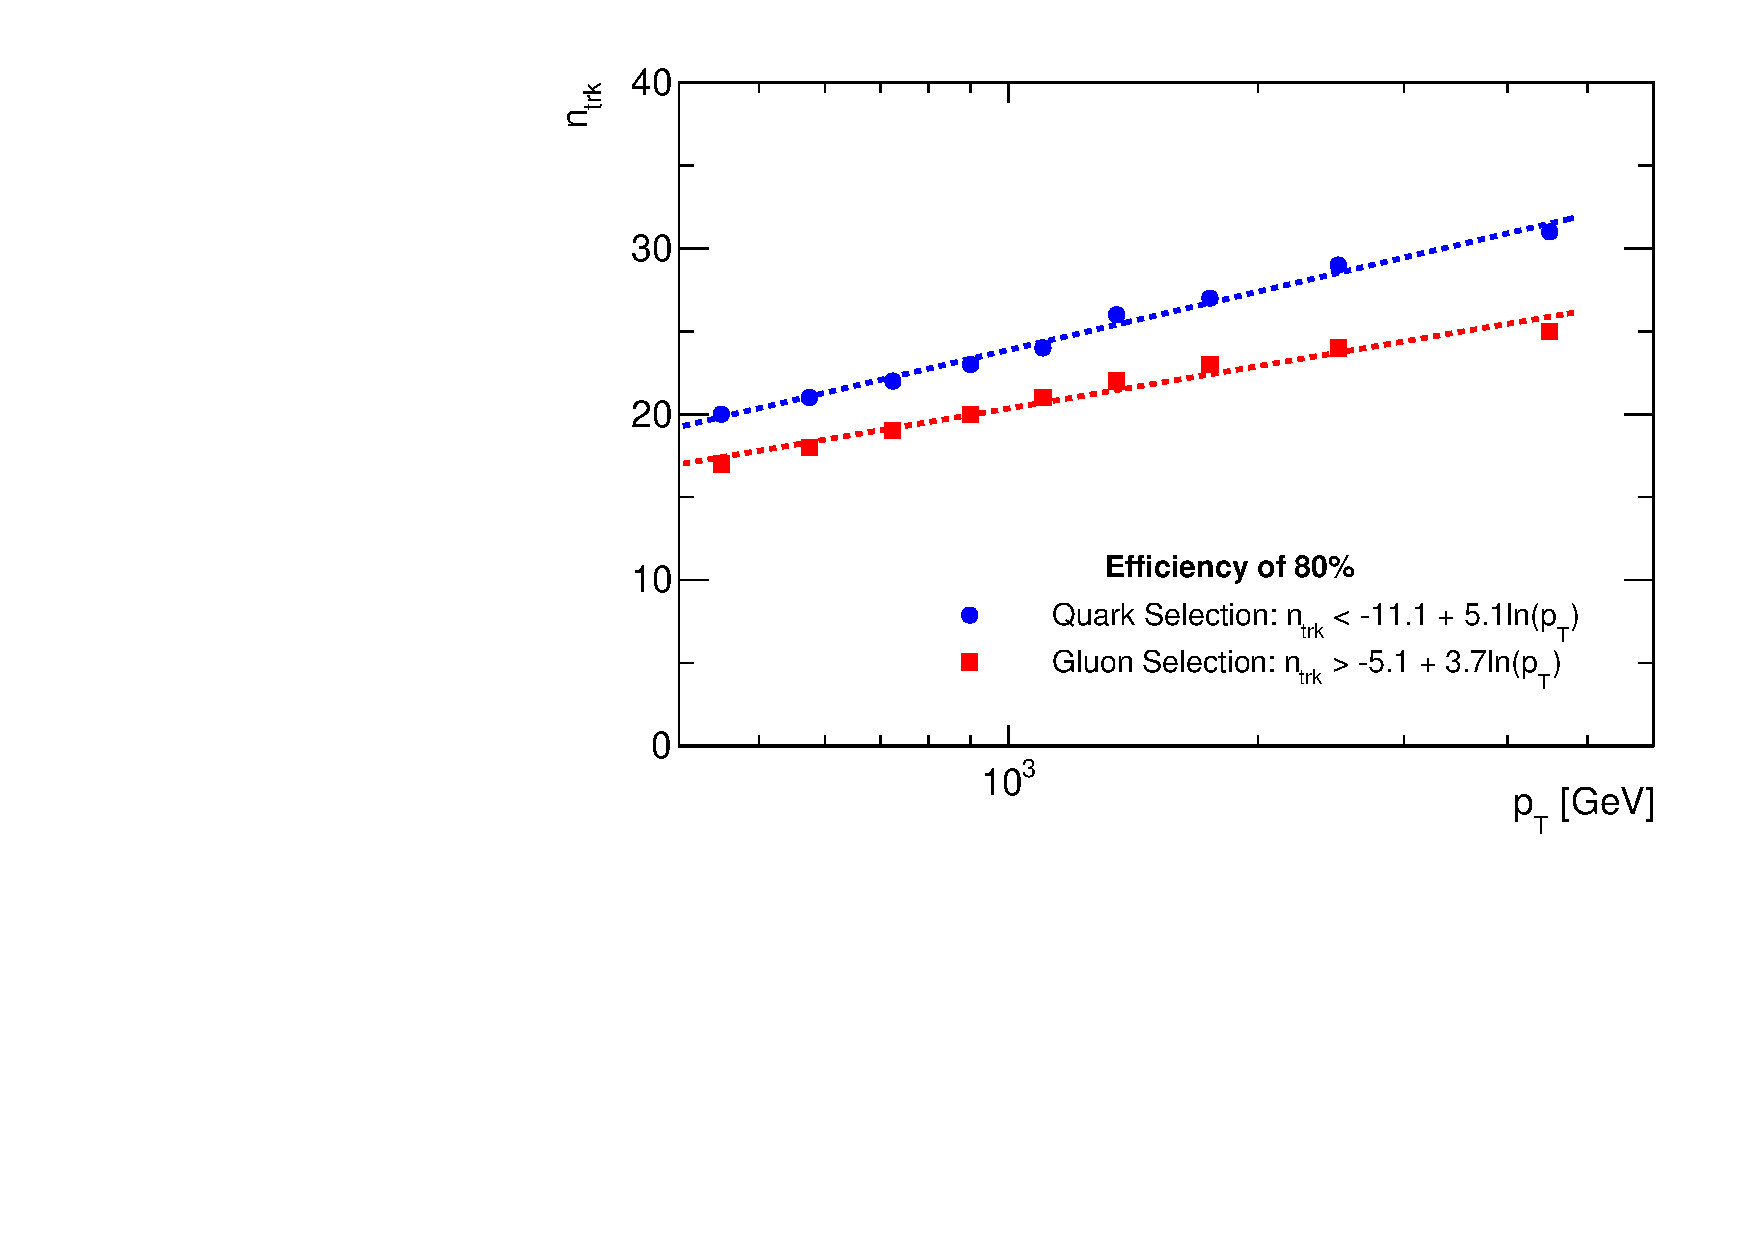
\includegraphics[width=0.495\textwidth]{figures/tagging/quark_selection_4}}

\caption{ The values of \ntrk\ for (a) 70\% and (b) 80\% quark (blue) and gluon (red) 
selection efficiencies in each \pT\ bin along with the best fit to Eq.~\ref{eq:nqg2}.
 \label{fig:qg_selection_curves}}
\end{figure}


\begin{table}[h]
	\centering 
		\caption{ Values of constants $m$ and $c$ from Eq.~\ref{eq:nqg2} such that $ \ntrk  \le \nq $ 
		for truth quark jets for a range of efficiencies  from 65 to 95\%. 
		\label{table:truthQuarkSelectionEfficiencies}
		}
	\begin{tabular}{SSSS}
	\toprule
\multicolumn{1}{c}{Truth-$q$ selection efficiency}   & \multicolumn{1}{c}{Truth-$g$ selection efficiency} &  \multicolumn{1}{c}{$c$}  &  \multicolumn{1}{c}{$m$} \\
\midrule 
0.95 & 0.73 & -20.0 & 7.7 \\
0.90 & 0.57 & -15.9 & 6.5 \\
0.85 & 0.45 & -13.1 & 5.6 \\
0.80 & 0.36 & -11.1 & 5.1 \\
0.75 & 0.28 & -9.1  & 4.5 \\
0.70 & 0.22 & -6.5  & 3.9 \\
0.65 & 0.18 & -4.4  & 3.5 \\
\bottomrule
\end{tabular}
\end{table}

\begin{table}[h]
	\centering 
		\caption{ Values of constants $m$ and $c$ from Eq.~\ref{eq:nqg2} such that $ \ntrk  \ge \ngluon $ 
		for truth quark jets for a range of efficiencies  from 65 to 95\%. 
		\label{table:truthGluonSelectionEfficiencies}
		}
	\begin{tabular}{SSSS}
	\toprule
\multicolumn{1}{c}{Truth-$g$ selection efficiency}   & \multicolumn{1}{c}{Truth-$q$ selection efficiency} &  \multicolumn{1}{c}{$c$}  &  \multicolumn{1}{c}{$m$} \\
\midrule 
0.95 & 0.59 & -3.9 & 2.7 \\
0.90 & 0.46 & -4.3 & 3.1 \\
0.85 & 0.39 & -5.4 & 3.5 \\
0.80 & 0.31 & -5.1 & 3.7 \\
0.75 & 0.27 & -7.3 & 4.2 \\
0.70 & 0.23 & -8.9 & 4.6 \\
0.65 & 0.20 & -8.0 & 4.6\\
\bottomrule
\end{tabular}
\end{table}


\subsection{Expected Signal Significance}

The dijet mass spectrum has a complex background with rapidly changing  fractions of events that originate 
from quark-quark, quark-gluon and gluon-gluon. The expected signal significance has been investigated using 
MC simulated  signals and background. The background is represented using the \QCD samples described 
in Section~\ref{qcdsamps}. 

\subsubsection{Signals that decay to quark-quark.}

The significance for signals that decay to a quark anti-quark pair are estimated using \Zprime\ models (Section~\ref{sec:Zprime}) using 
\begin{equation}
S = N_S \sum_i{ \dfrac{ f_{{qq}_i}\epsilon_{qQ}^2 + f_{{qg}_i}\epsilon_{qQ}\epsilon_{gQ} + f_{{gg}_i}\epsilon_{gQ}^2  } {\sqrt{ B_{{qq}_i}\epsilon_{qQ}^2 + B_{{qg}_i}\epsilon_{qQ}\epsilon_{gQ} + B_{{gg}_i}\epsilon_{gQ}^2  }}}
\end{equation}
where $N_S$ is the number of signal events, $f_{{qq}_i}$ is fraction of signal events that result in the two 
highest \pT\ jets that where initiated by quarks in bin $i$ ( $f_{{qg}_i}$ are quark-gluon jets, and $f_{{gg}_i}$ is two gluon jets), 
$\epsilon_{qQ}$ is the efficiency of a quark initiated jet passing the quark selection criteria, 
$\epsilon_{gQ}$ is the efficiency of a gluon initiated jet passing the quark selection criteria, 
and $B_{{xx}_i}$ is the expected number of background events with quark-quark, quark-gluon or gluon-gluon initiated jets. 


The significance is calculated for \Zprime's with masses ranging from 1500 to 4000\,\GeV and quark-jet selection 
efficiencies ranging from 30 to 90\%. The resulting significances are  in Fig.~\ref{fig:QuarkSignalSignificance}
and show that the significance decreases if any quark-selection is applied to the data. This is because
the data is dominated by quark-quark events and the selection reduces background and signal in similar amounts. 

\begin{figure}[htb]
 \centering
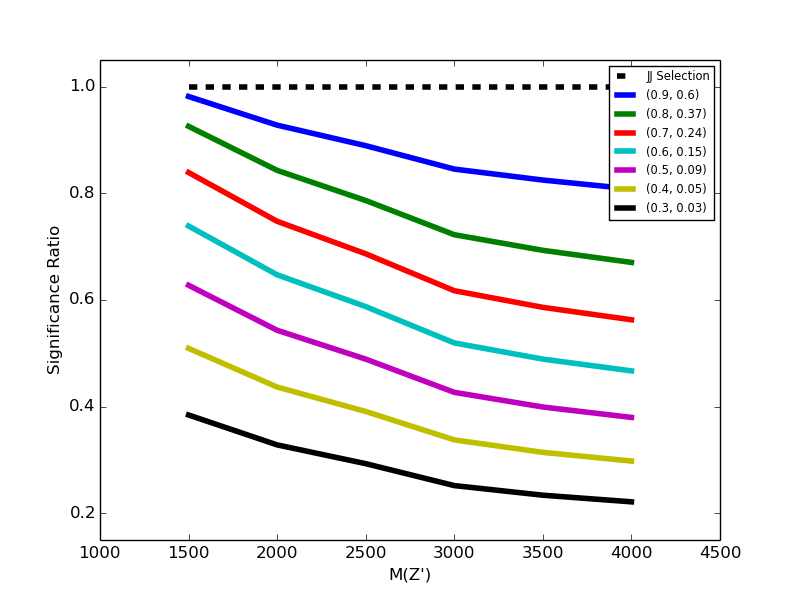
\includegraphics[width=0.75\textwidth]{figures/tagging/QuarkSignalSignificance.png}
\caption{ The significance for observing a \Zprime\ with masses from 1500 to 4000\,\GeV
for $\epsilon_{qQ}$ ranging from 90 to 30\% compared to the significance calculated with no quark selection applied. The key gives pairs of efficiencies ($\epsilon_{qQ}$, $\epsilon_{gQ}$).
  \label{fig:QuarkSignalSignificance}}
\end{figure}

\subsubsection{Signals that decay to gluon-gluon.}

The significance for signals that decay to a gluon-gluon pair are estimated using \Hprime\ models  using 
\begin{equation}
S = N_S \sum_i{ \dfrac{ f_{{qq}_i}\epsilon_{qG}^2 + f_{{qg}_i}\epsilon_{qG}\epsilon_{gG} + f_{{gg}_i}\epsilon_{gG}^2  } {\sqrt{ B_{{qq}_i}\epsilon_{qG}^2 + B_{{qg}_i}\epsilon_{qG}\epsilon_{gG} + B_{{gg}_i}\epsilon_{gG}^2  }}}
\end{equation}
where  
$\epsilon_{qG}$ is the efficiency of a quark initiated jet passing the gluon selection criteria, 
$\epsilon_{gG}$ is the efficiency of a gluon initiated jet passing the gluon selection criteria. 
The significance is calculated for \Hprime's with masses ranging from 2000 to 7000\,\GeV\ and quark-jet selection 
efficiencies ranging from 60 to 90\%. The resulting significances are  in Fig.~\ref{fig:GluonSignalSignificance}
and show that the significance increases from approximately 1.2 at 2\,TeV\ to 1.6 at 7\,\TeV\ with the greatest 
increases  occurring for gluon selection efficiency of 75\%. 

\begin{figure}[htb]
 \centering
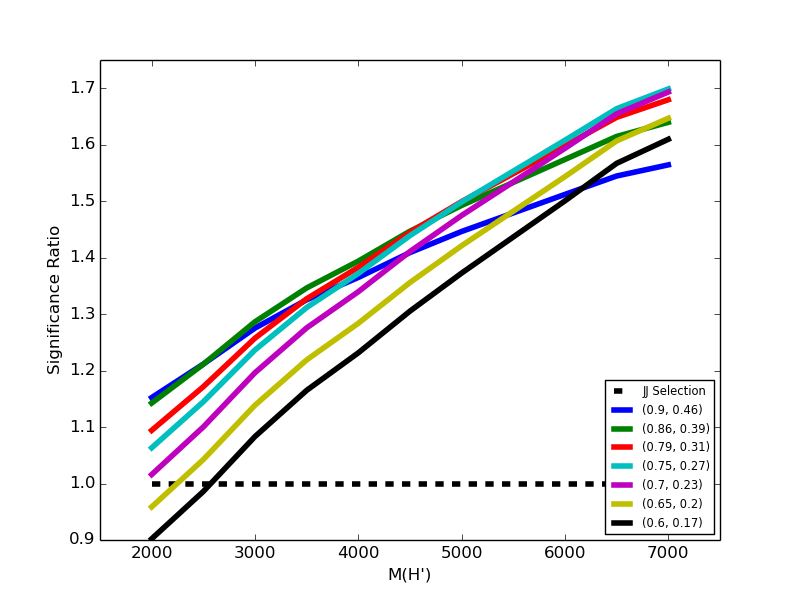
\includegraphics[width=0.75\textwidth]{figures/tagging/GluonSignalSignificance.png}
\caption{ The significance for observing a \Hprime\ with masses from 2000 to 7000\,\GeV\ 
for $\epsilon_{gG}$ ranging from 90 to 60\% compared to the significance calculated with no gluon selection applied. The key gives pairs of efficiencies ($\epsilon_{gG}$, $\epsilon_{qG}$).
  \label{fig:GluonSignalSignificance}}
\end{figure}


\subsubsection{Signals that decay to quark-gluon.}


The calculation of the significance for a quark-gluon signal such as an excited quark decay is much more complicated as 
both jets can satisfy both the quark and the gluon selection.  In this case we need to define three efficiencies that are exclusive for quark and gluon jets. They are 
\begin{itemize}
\item $\epsilon_{qQ}$ The probability that a quark initiated jet is identified only as a quark jet. 
\item $\epsilon_{qQG}$ The probability that a quark initiated jet is identified  as a quark and a gluon jet.
\item $\epsilon_{qG}$ The probability that a quark initiated jet is identified only as a gluon jet.  
\end{itemize}
where by construction $\epsilon_{qQ} + \epsilon_{qQG} + \epsilon_{qG} = 1$. A similar set of efficiencies are measured 
for gluon initiated jets. 
\begin{itemize}
\item $\epsilon_{gQ}$ The probability that a gluon initiated jet is identified only as a quark jet. 
\item $\epsilon_{gQG}$ The probability that a gluon initiated jet is identified  as a quark and a gluon jet.
\item $\epsilon_{gG}$ The probability that a gluon initiated jet is identified only as a gluon jet.  
\end{itemize}

The probability of truth quark-quark ($p_{qq}$), quark-gluon ($p_{qg}$) and gluon-gluon ($p_{gg}$) truth 
events of passing the selection criteria are given by 
\begin{align}
p_{qq} & = 2  \epsilon_{qQ}\epsilon_{qG} + \epsilon_{qQG}\left( \epsilon_{qQ} + \epsilon_{qG} \right)  + \epsilon_{qQG}\epsilon_{qQG} \\
p_{gg} & = 2  \epsilon_{gQ}\epsilon_{gG} + \epsilon_{gQG}\left( \epsilon_{gQ} + \epsilon_{gG} \right)  + \epsilon_{gQG}\epsilon_{gQG} \\
p_{qg} & = \epsilon_{qQ}\epsilon_{gG} + \epsilon_{gQ}\epsilon_{qG} + \epsilon_{qQG}\left( \epsilon_{gQ} + \epsilon_{gG} \right) 
+ \epsilon_{gQG}\left( \epsilon_{qQ} + \epsilon_{qG} \right) 
+ \epsilon_{gQG}\epsilon_{gQG}
\end{align}
and the significance is then given by 
\begin{equation}
S = N_S \sum_i{ \dfrac{ f_{{qq}_i} p_{qq} + f_{{qg}_i}p_{qg} + f_{{gg}_i}p_{gg}  } {\sqrt{ B_{{qq}_i}p_{qq} + B_{{qg}_i}p_{qg} + B_{{gg}_i}p_{gg}  }}}.
\end{equation}

Exploring selection efficiencies from 30 to 100\% for both quarks and gluons shows that no benefit 
is obtained by applying a quark selection. A small but significant improvement in significance is obtained 
if one of the two jets is required to pass a gluon selection. The resulting significances are  in Fig.~\ref{fig:QuarkGluonSignalSignificance}
and show that the significance increases by about 25\% at high masses (above 5\,\TeV ) with the greatest 
increases  occurring for gluon selection efficiency over 70\%. 


\begin{figure}[htb]
 \centering
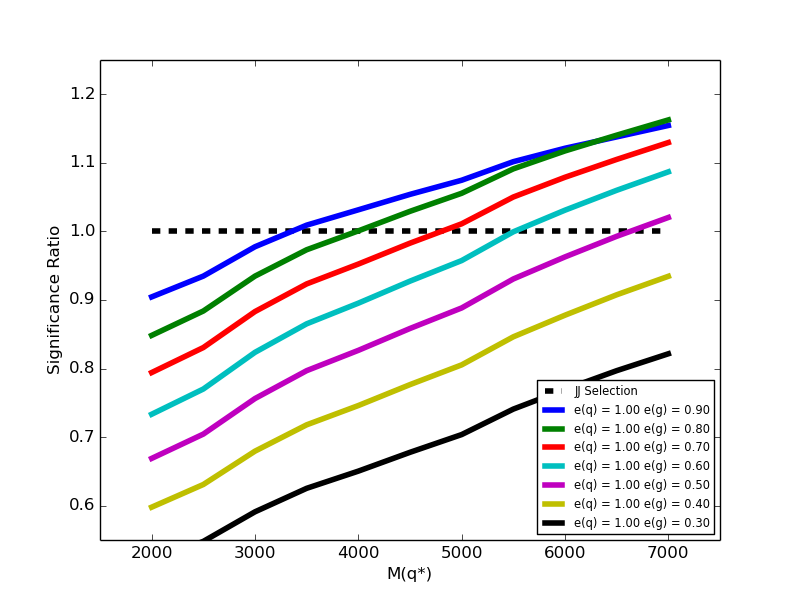
\includegraphics[width=0.75\textwidth]{figures/tagging/QuarkGluonSignalSignificance3.png}
\caption{ The significance for observing a \qstar\ with masses from 2000 to 7000\,\GeV\ 
for $\epsilon_{gG}$ ranging from 30 to 90\% compared to the significance calculated with no gluon selection applied. The key gives pairs of efficiencies ($\epsilon_{gG}$, $\epsilon_{qG}$).
  \label{fig:QuarkGluonSignalSignificance}}
\end{figure}


%\begin{equation}
%S = N_S \sum_i{ \dfrac{ f_{{qq}_i}\epsilon_{qG}^2 + f_{{qg}_i}\epsilon_{qG}\epsilon_{gG} + f_{{gg}_i}\epsilon_{gG}^2  } {\sqrt{ B_{{qq}_i}\epsilon_{qG}^2 + B_{{qg}_i}\epsilon_{qG}\epsilon_{gG} + B_{{gg}_i}\epsilon_{gG}^2  }}}
%\end{equation}
%
%
%
%Two alternative
%selection criteria have been investigated, one based on that used in
%Ref.~\cite{ATL-PHYS-PUB-2017-009} and a simple linear alternative. A jet
%is classed as being quark-initiated if \ntrk is less than the threshold
%\nqg\ (Eq.~\ref{eq:QGselect}):

%These selection criteria are applied to the two leading jets to separate dijet events into three samples:
%where both jets are more likely to be quark-initiated, \QQ,  where both jets are more likely to
%be gluon-initiated, \GG, and where we have one of each, \QG.
%Simulated background events are separated into sub-samples based on the selection criteria given in
%Eqs.~\ref{eq:nqg1} and \ref{eq:nqg2} and are shown in Fig.~\ref{fig:pythia_qg_selection}. It is clear that
%the selection using Eq.~\ref{eq:nqg1} (Fig.~\ref{fig:pythia_qg_selection} a) produces more complex background shapes
%than those Eq.~\ref{eq:nqg2} (Fig.~\ref{fig:pythia_qg_selection} b). Since the selection using  Eq.~\ref{eq:nqg2} will
%be much easier to fit it will be used for initial toy-MC studies of limit setting. Alternative selections using Eq.~\ref{eq:nqg2} are produced for comparison, "selection 1" with m = 0.02, c = 0, and "selection 4" with m = 0.01, c = 15.

%
%
%Figure~\ref{fig:QG_qstar_4tev} shows the selection applied to the mass distribution of a 4\,TeV \qstar . The  
%\QQ sample is more peaked and has a smaller tail than the \QG\ distribution which has a similar shape to the complete signal. The \GG\ sample of high multiplicity jets has a very small peak and is dominated by the tail.
%
%\begin{figure}[htb]
% \centering
%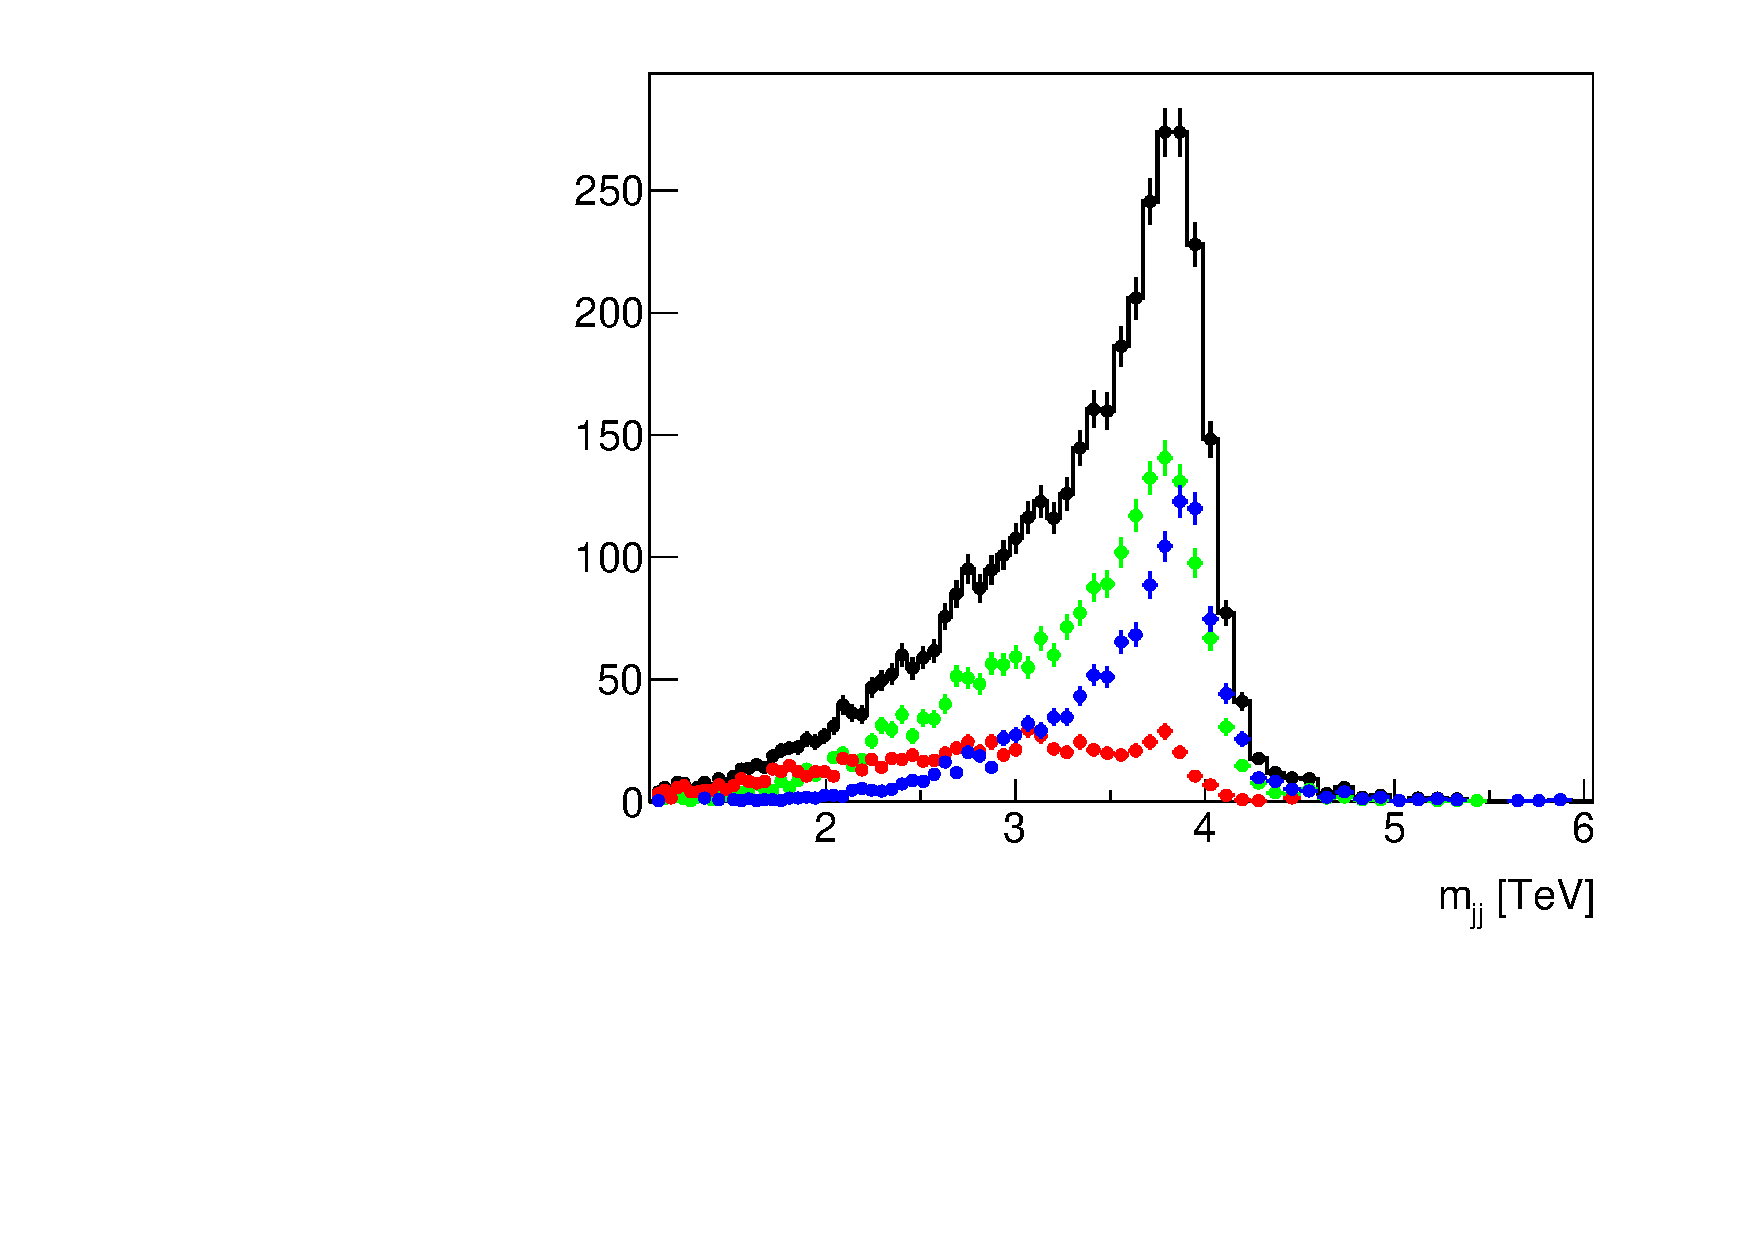
\includegraphics[width=0.75\textwidth]{figures/tagging/QG_qstar_4tev.pdf}
%\caption{Simulated 4\,TeV \qstar\ sample seperated into \QQ\ (blue) , \QG\ (green) and \GG\ (red) 
%sub-samples.  \label{fig:QG_qstar_4tev}}
%\end{figure}
%
%\clearpage
%\subsection{Signal Fractions Quark-Gluon selection}
%
%The fraction of \qstar\ signal events is measured for masses from 1\,TeV to 7.0\,TeV and are given in Table~\ref{table:qstar_fractions}. The low fraction of \QQ\ events at masses from 1 to 3\,TeV suggest that
%further optimisation of the selection criteria are required.  
%
%\begin{table}[h]
%	\centering 
%		\caption{The fraction of \qstar\ MC events in the \QQ, \QG, and \GG\ sub-samples for various masses. 
%		\label{table:qstar_fractions}}
%	\begin{tabular}{SSSS}
%	\toprule
%\qstar\ Mass (TeV) & \multicolumn{1}{c}{\QQ\ Fraction} &  \multicolumn{1}{c}{\QG\ Fraction}  &  \multicolumn{1}{c}{\GG\ Fraction} \\
%\midrule 
%1.0	&	0.06 &	0.31 &	0.63\\
%2.0	&	0.04 &	0.37 &	0.59\\
%2.5	&	0.09 &	0.45 & 	0.46\\
%3.0	&	0.15 &	0.51 &	0.35\\
%3.5	&	0.22 &	0.53 &	0.25\\
%4.0	&	0.30 &	0.51 &	0.19\\
%4.5	&	0.37 &	0.48 &	0.15\\
%5.0	&	0.44 &	0.44 &	0.12\\
%5.5	&	0.49 &	0.41 &	0.10\\
%6.0	&	0.53 &	0.37 &	0.09\\
%6.5	&	0.56 &	0.35 &	0.09\\
%7.0	&	0.57 &	0.33 &	0.10\\
%\bottomrule
%\end{tabular}
%\end{table}
%
%
%\begin{figure}[htb]
% \centering
%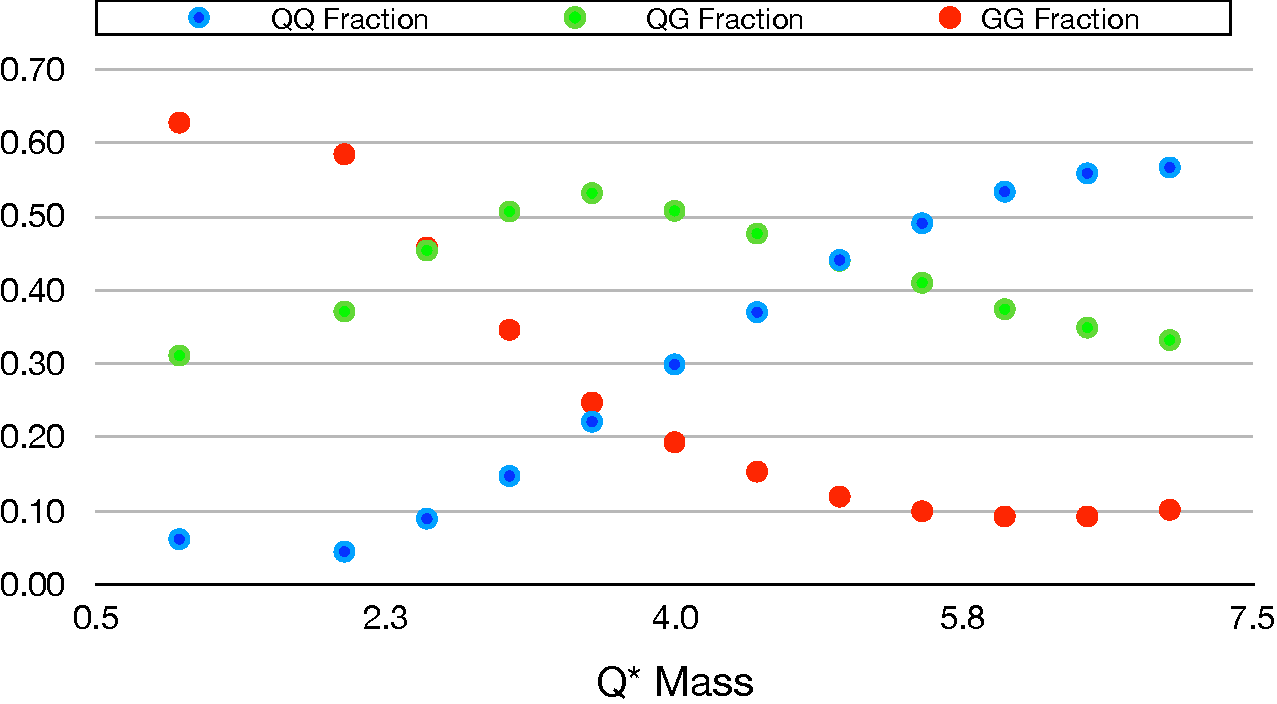
\includegraphics[width=0.75\textwidth]{figures/tagging/QStarEfficincies.pdf}
%\caption{The fraction of \qstar\ MC events in the \QQ, \QG, and \GG\ sub-samples for various masses.   \label{fig:QStarEfficincies}}
%\end{figure}
%
%
%
%\subsection{Signal Morphing with Quark-Gluon selection}
%
%Signal morphing (Sec.\ref{sec:SwiftMorphing}) is applied to the \qstar\ signal subsamples. The MC signal 
%sub-samples for \QQ\ and \QG\ are fit to a Gaussian + reverse Landau function, a parameterization that has 
%one normalization  and five shape parameters. The parameters are interpolated as a function of mass using cubic splines.
%%\textit{ \color{red} The \GG\ subsamples have not been morphed at this time.} 
%
